%%%%%%%%%%%%%%%%%%%%%%%%%%%%%%%%%%%%%%%%%
% Journal Article
% LaTeX Template
% Version 2.0 (February 7, 2023)
%
% This template originates from:
% https://www.LaTeXTemplates.com
%
% Author:
% Vel (vel@latextemplates.com)
%
% License:
% CC BY-NC-SA 4.0 (https://creativecommons.org/licenses/by-nc-sa/4.0/)
%
% NOTE: The bibliography needs to be compiled using the biber engine.
%
%%%%%%%%%%%%%%%%%%%%%%%%%%%%%%%%%%%%%%%%%

%%%%%%%%%%%%%%%%%%%%%%%%%%%%%%%%%%%%%%%%%
% template adapted for use in the KU Leuven course on science communication (physics and mathematics)
%%%%%%%%%%%%%%%%%%%%%%%%%%%%%%%%%%%%%%%%%


%----------------------------------------------------------------------------------------
%	PACKAGES AND OTHER DOCUMENT CONFIGURATIONS
%----------------------------------------------------------------------------------------

\documentclass[
a4paper, % Paper size, use either a4paper or letterpaper
10pt, % Default font size, can also use 11pt or 12pt, although this is not recommended
unnumberedsections, % Comment to enable section numbering
twoside, % Two side traditional mode where headers and footers change between odd and even pages, comment this option to make them fixed
]{LTJournalArticle_JS}
\usepackage{newtxtext}
\usepackage{amsmath}
\usepackage{float}
\usepackage{hyperref}
\usepackage{graphicx}
\usepackage{wrapfig}
\usepackage{siunitx}
\usepackage{csquotes}
\addbibresource{sample.bib} % BibLaTeX bibliography file

\runninghead{Chaotic Behaviour of a Double Pendulum} % A shortened article title to appear in the running head, leave this command empty for no running head

\footertext{\textit{Bachelor Journal of Science Communication: Physics} (2026) Vol 3} % Text to appear in the footer, leave this command empty for no footer text

\setcounter{page}{1} % The page number of the first page, set this to a higher number if the article is to be part of an issue or larger work

%----------------------------------------------------------------------------------------
%	TITLE SECTION
%----------------------------------------------------------------------------------------

\title{Theoretical vs. Experimental Dynamics of a \\ Double Pendulum: Trajectory Comparison \\ and Lyapunov Characterization} % Article title, use manual lines breaks (\\) to beautify the layout

% Authors are listed in a comma-separated list with superscript numbers indicating affiliations
% \thanks{} is used for any text that should be placed in a footnote on the first page, such as the corresponding author's email, journal acceptance dates, a copyright/license notice, keywords, etc
\author{%
	Baselmans Quinten\textsuperscript{1} and Swinnen Nand\textsuperscript{2}
}
\renewcommand{\prependtopagenr}{r1039544 \& r1049998 - } %insert your student-number. Leave the - at the end. 
% Affiliations are output in the \date{} command
\date{\footnotesize\textsuperscript{\textbf{1}}Bachelor of Physics, minor Biochemistry, KU Leuven\\ \textsuperscript{\textbf{2}}Bachelor of Physics, minor Astronomy, KU Leuven}

% Full-width abstract
\renewcommand{\maketitlehookd}{
\begin{abstract}
	The double pendulum is a textbook example of a chaotic system, exhibiting strong sensitivity to initial conditions. This study investigates whether the theoretical dynamics, chaos and initial condition dependence of a double pendulum translate to an experimental setting. A double pendulum was constructed with optimised, low-friction bearings to minimize energy dissipation, and its motion was tracked and compared against a numerical simulation. Chaotic behaviour was further examined by comparing experimental outcomes with the double pendulum fractal. Results indicate that while friction causes eventual trajectory divergence after $t_{div} = (0.3 \pm 0.2) \ \unit{s}$, the underlying chaotic behaviour remains consistent with theory, highlighting that its chaotic character is fundamentally inherent to the system.
\end{abstract}
}

%----------------------------------------------------------------------------------------

\begin{document}
\maketitle % Output the title section
%----------------------------------------------------------------------------------------
%	ARTICLE CONTENTS
%----------------------------------------------------------------------------------------
\section{Introduction}
The dynamics of the masses of a double pendulum form a complex system, characterised by pronounced sensitivity to initial conditions on the paths of motion. This system has been extensively studied in theory, but how does this dependence on initial conditions fare in a non-ideal experiment, and how accurate are the theoretical paths of the masses? The aim of this paper is to compare the theoretical (Lagrangian) and experimental motion of the masses, and to investigate the extent to which chaotic sensitivity to initial conditions is observed in practice.
%------------------------------------------------
\section{Theory}

A standard double pendulum is a two-dimensional frictionless system with massless rods and masses on their ends. An example is pictured in \autoref{fig:DP}. The motion of the angles $\theta_1$ and $\theta_2$ as a function of time are given by the Lagrangian equations of motion (EOM), for $\theta_1$ and $\theta_2$ respectively \cite{EOM}:
\begin{equation}\label{EOM}
	\left\{
	\begin{aligned}
		& m_2 L_1 L_2 \dot{\theta}_2^2 \sin(\theta_2 - \theta_1) 
		+ (m_1 + m_2) g L_1 \sin(\theta_1) \\
		&= (m_1 + m_2) L_1^2 \ddot{\theta}_1 
		- m_2 L_1 L_2 \ddot{\theta}_2 \cos(\theta_2 - \theta_1) \\
		& m_2 L_1 L_2 \dot{\theta}_1^2 \sin(\theta_2 - \theta_1) 
		+ m_2 g L_2 \sin(\theta_2) \\
		&= -\left( m_2 L_2^2 \ddot{\theta}_2 
		+ m_2 L_1 L_2 \ddot{\theta}_1 \cos(\theta_2 - \theta_1) \right)
	\end{aligned}
	\right.
\end{equation}

In these equations, $m_1$ and $m_2$ are the first and second masses, $L_1$ and $L_2$ the lengths of the rods and $g = 9.81 \ \unit{m.s^{-2}}$ is the gravitational acceleration (\autoref{fig:DP}). Given the initial conditions, representing the angles and their angular speeds at $t = 0 \ \unit{\second}$ $(\theta_1(0), \theta_2(0), \omega_1(0), \omega_2(0))$, these coupled equations can be solved to predict the theoretical path of the masses.

\begin{figure}[H]
	\centering
	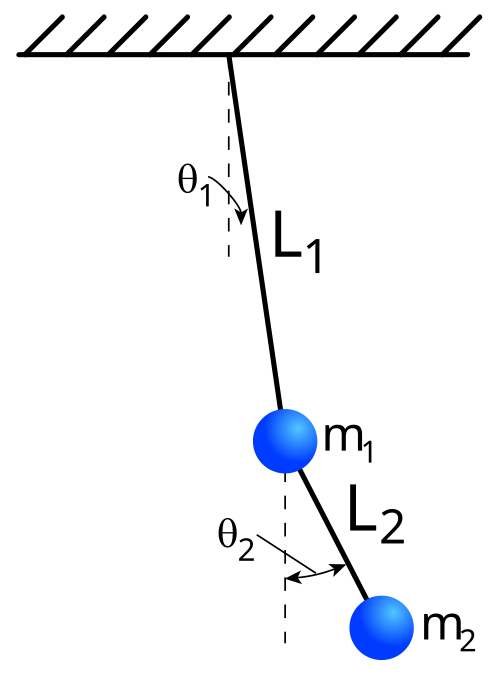
\includegraphics[width = 0.45\linewidth]{Figures/Double-Pendulum.png}
	\caption{A model of a double pendulum \cite{Wikipedia-afbeelding}.}
	\label{fig:DP}
\end{figure}
The kinetic energy $K$ and the potential energy $V$ of the system are calculated with \cite{KlasMech}:
\[
\begin{aligned}
	V &= -gm_1 L_1\cos(\theta_1) -gm_2(L_1 \cos(\theta_1) + L_2 \cos(\theta_2)) \\
	K &= \frac{1}{2}m_1(L_1 \dot{\theta}_1)^2 + {} \\
	&\quad \ \  \frac{1}{2}m_2\left( (L_2 \dot{\theta}_2)^2 + (L_1 \dot{\theta}_1)^2 + 2 L_1L_2 \cos(\theta_2 - \theta_1) \dot{\theta}_1\dot{\theta}_2 \right)
\end{aligned}
\]

Visually, chaos occurs when nearby initial conditions produce diverging trajectories. Quantitatively, chaos is calculated by the Lyapunov-exponent $\lambda$. This number quantifies the rate at which initially close trajectories diverge \cite{lyup}. The faster they diverge, the more chaotic that starting angle is. A double pendulum fractal is a graph that displays $\lambda$ for several initial conditions.

In this experiment, $\lambda$ is calculated in the four-dimensional phasespace ($\theta_1, \theta_2, \omega_1, \omega_2$), with an offset of $\varepsilon=10^{-9} \ \unit{rad}$ for the starting angles in the simulations. When $\lambda >0 \ \unit{s^{-1}}$, the system is classified as chaotic. The simulations, however, use $\lambda > 0.25 \ \unit{s^{-1}}$ as a threshold for chaos to account for numerical artifacts.
%------------------------------------------------
\section{Methodologies}
For this study, a double pendulum was constructed and its motion was filmed using a slow motion camera. These videos were tracked using the software `Tracker' \cite{tracker}. The experimental pendulum is visible in \autoref{fig:reality}.

\begin{figure}[H]
	\centering
	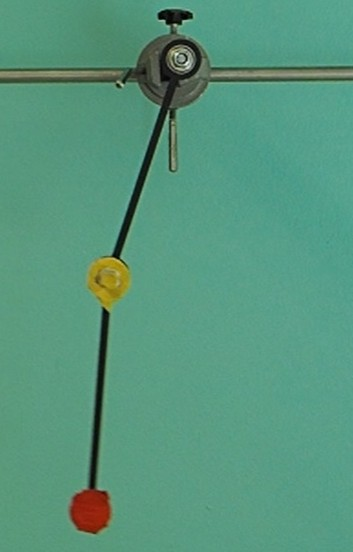
\includegraphics[width=0.45\linewidth]{Figures/onze_pendulum.jpeg}
	\caption{The pendulum that was used in the experiment, with the masses at the end colored to simplify the tracking process.}
	\label{fig:reality}
\end{figure}

To better match the theoretical model, lightweight plastic rods were 3D-printed. In the pivoting points, ball bearings were installed to minimize friction. They also served as the masses, and the bottom mass also is a ball bearing for consistency. The error on the tracking process is caused by inaccuracies with the program looking for the exact midpoint of the mass, as well as frames that needed to be tracked manually.

The theoretical trajectories were obtained by integrating the EOM (\ref{EOM}) using the Runge-Kutta method \cite{RK4}, using the experimental initial angles and initial speeds of zero. The bulk of this simulation is based on an article from Scipython \cite{simulation}. The EOM were solved for the specific case of the pendulum, with $L_1 = L_2 = (16.5 \pm 0.2) \ \unit{cm}$, $m_1 = (69 \pm 1) \ \unit{g}$ and $m_2= (20 \pm 1) \ \unit{g}$. A Lyapunov fractal (\autoref{fig:fractal}) was also constructed for various starting angles.

Chaotic behaviour in the experimental data was assessed by evaluating whether the bottom mass performs a complete ($360^\circ$) rotation. At these angles, the linear approximation of the EOM falls apart, making the motion non-periodic as $t \to \infty$ \cite{journalofphysics}.

%------------------------------------------------

\section{Results}
\autoref{fig:mooie figuur} compares the theoretical and experimental trajectories of the second mass from one of the experiments, where it is visible that it follows the theoretical model initially, but eventually diverges. The `time of divergence' is defined as the moment at which the angular separation between the theoretical and experimental path exceeds, on average, the error on the data on three consecutive frames. For the 32 tracked trajectories, the average time of divergence is $t_{div} = (0.3 \pm 0.2) \ \unit{s}$. The second graph shows the kinetic and potential energy and their resulting total energy $E = K + V$.

Secondly, in the double pendulum fractal shown in \autoref{fig:fractal}, dots of the tracked data were added. The dots are blue if the bottom mass made a full turn (chaotic) and green if it did not (non-chaotic).
\begin{figure}[H]
	\centering
	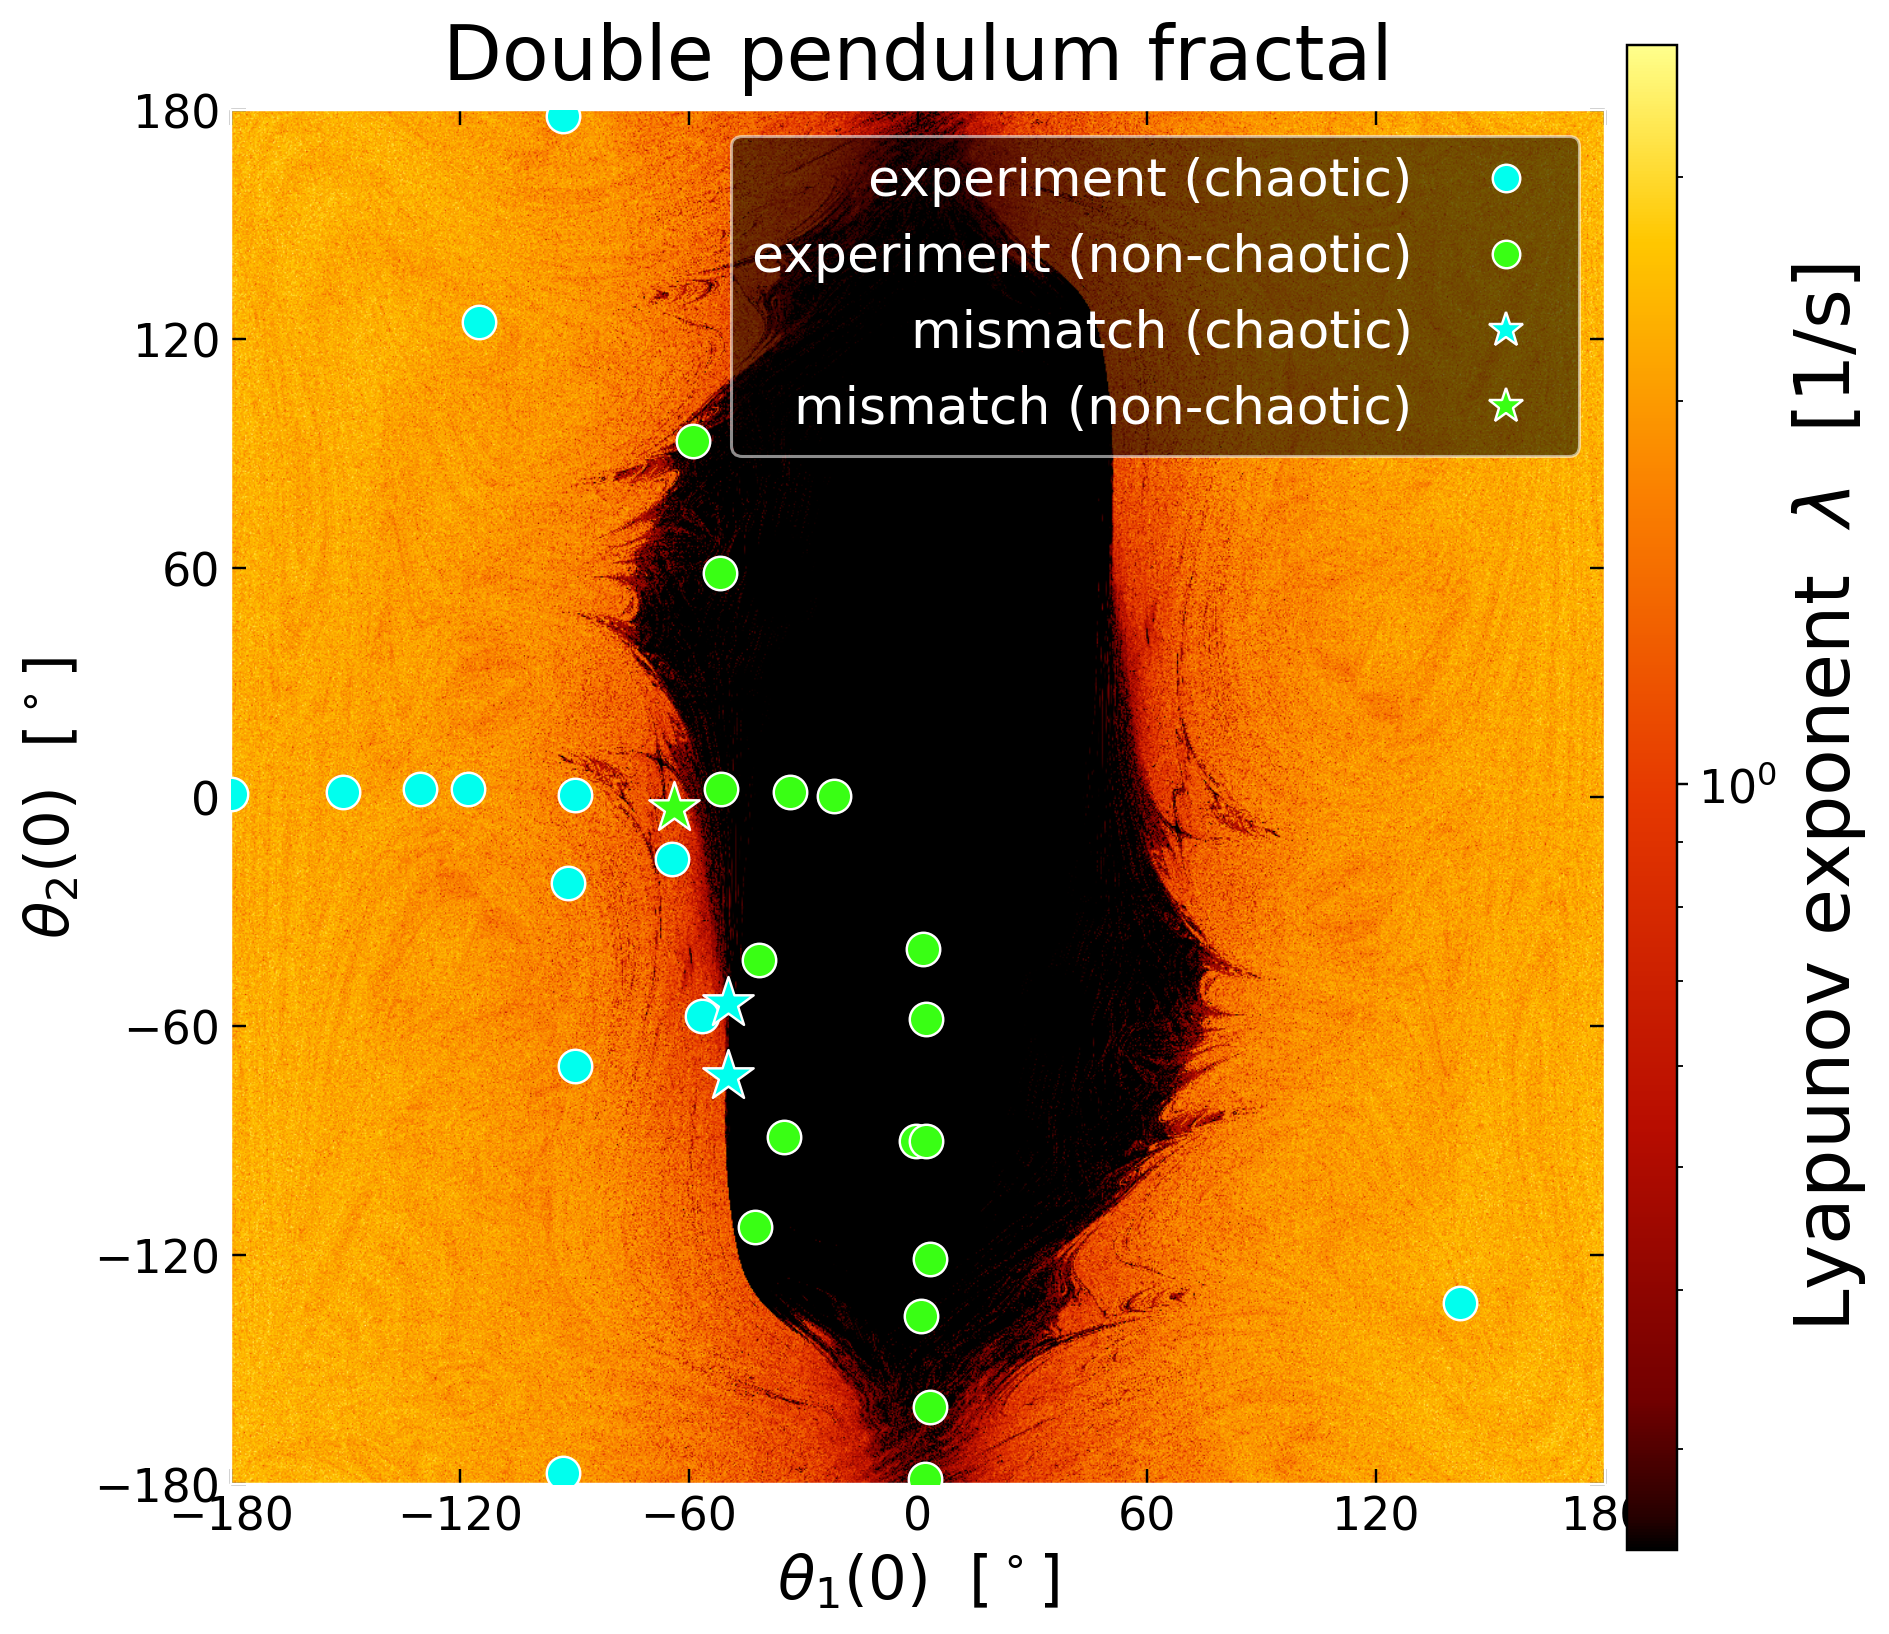
\includegraphics[width=1\linewidth]{Figures/eigen_chaos_kaart.png}
	\caption{The double pendulum fractal, simulated with the parameters of the real pendulum. Black areas are non-chaotic starting angles, and the others are chaotic. Experimental data is added as the colored dots.}
	\label{fig:fractal}
\end{figure}
%------------------------------------------------
\section{Discussion}
As expected, experimental trajectories rapidly diverge from the ideal Lagrangian EOM (\ref{EOM}) predictions. This divergence is primarily driven by internal friction in the bearings, air drag and a 'wobbling' perpendicular to the plane of motion, which cause energy dissipation in the experimental pendulum. Minor numerical integration errors in the simulations also cause possible discrepancy. However, the experimental path does follow the general trends of the simulation for a longer time, before eventually being completely different as well. 

The fractal shows that the experimental data is (non-) chaotic where predicted, with the theory and results agreeing closely aside from a few edge cases (marked with a star in \autoref{fig:fractal}). These edge cases can, again, be explained by external effects not included in the simulations. 

For following research, friction in the ball bearings could be calculated and both rods could be seen as a rigid body. These could then be compared to EOM that account for these factors, as seen, for example, in \cite{friction}.
\begin{figure*}[t]
	\centering
	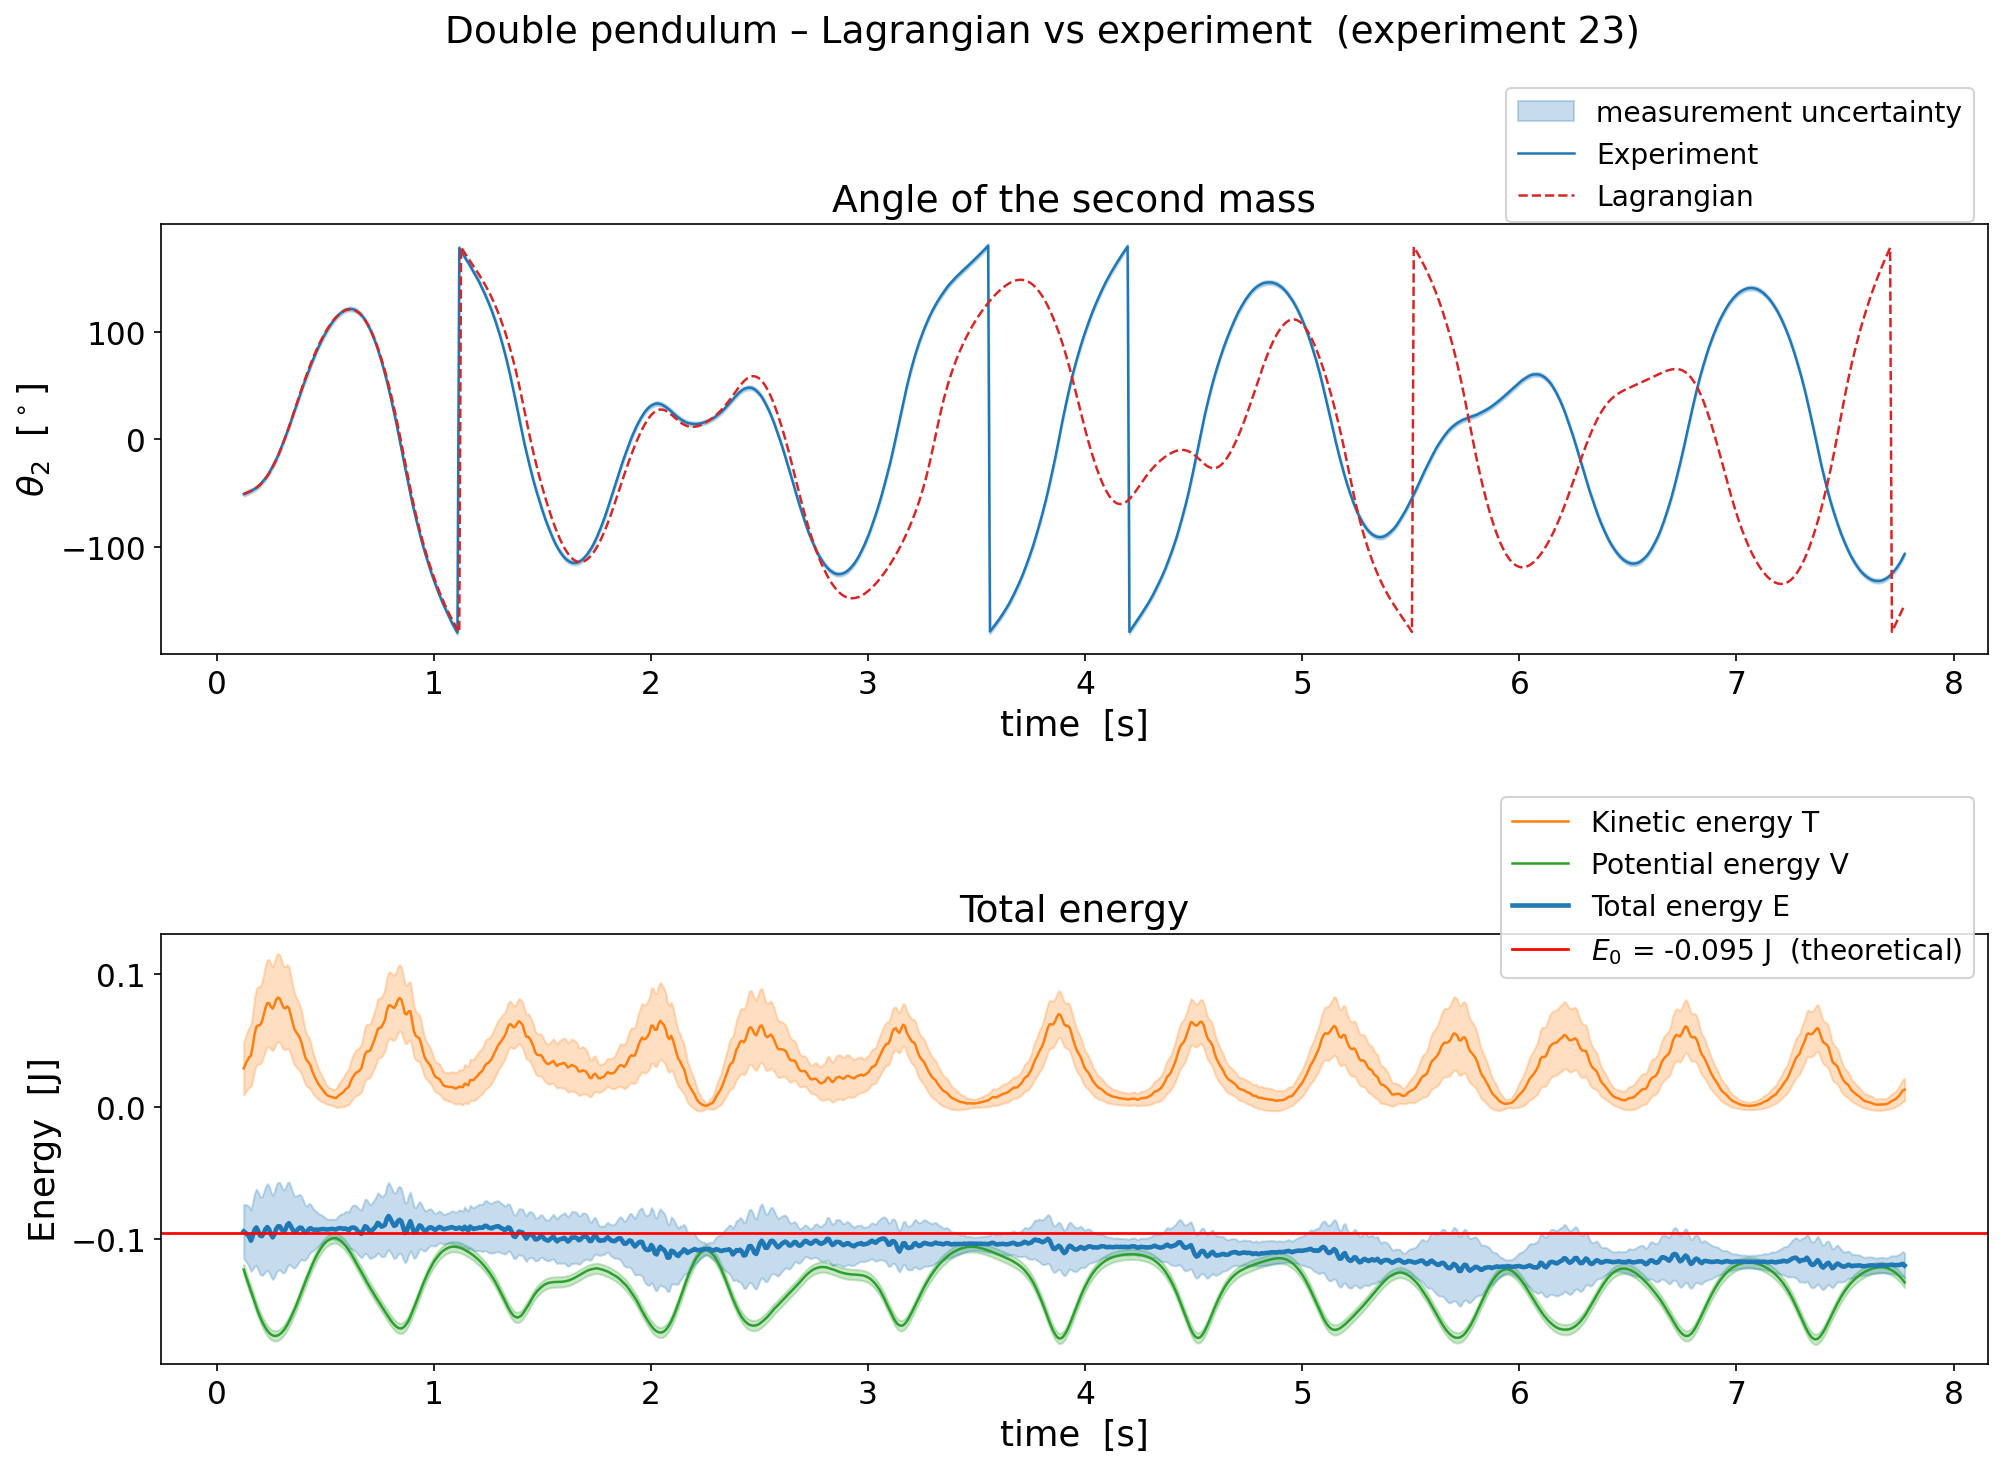
\includegraphics[width= 0.75\linewidth]{Figures/dubbele_slinger_23.png}
	\caption{The evolution of $\theta_2(t)$ and the total energy of the system, with errors that are due to inaccuracies of the tracker, with $\sigma_\theta = 1.9^\circ$, and errors that are due to error propagation of the angles, the masses and the lengths of the rods.}
	\label{fig:mooie figuur}
\end{figure*}
\section{Conclusion}
In general, the predicted path of the masses and the experimental path match shortly, but after that they diverge due to effects of friction and drag taking over. Chaotic behaviour, on the other hand, matches the theory overall and is thus inherent for the double pendulum. For more accurate results, EOM that include friction can be used for future research.

%----------------------------------------------------------------------------------------
%	 REFERENCES
%----------------------------------------------------------------------------------------

\printbibliography % Output the bibliography

%----------------------------------------------------------------------------------------

\end{document}
